\label{sec:trkperf}


In order to study the tracking performance of the detector, we use samples of $A'$ events 
at a variety of energies and decay lengths.  On top of each event, we overlay backgrounds 
produced by the passage of  beam electrons equivalent to our optimized run conditions at
different beam energies and with a W target and a beamspot of Gaussian sigma of 40$\mu$m in the vertical direction and 
200$\mu$m in the horizontal. The beam energies, currents, target thickness and analyzing magnetic field  used for these simulations are:
\begin{itemize}
\item 50nA at 1.1 GeV with $X_0=0.125$\% and  B=0.25 T
\item 200nA at 2.2 GeV with $X_0=0.125$\% and  B=0.5 T
\item 300nA at 4.4 GeV with $X_0=0.25$\% and  B=1.0 T
\item 450nA at 6.6 GeV with $X_0=0.25$\% and  B=1.5 T
\end{itemize}
At each energy, we evaluate momentum, invariant mass, and vertex resolution.  The plots shown in the following section typically use the 4.4 GeV beam as an example.  

\subsection{Tracking Efficiency, Pattern Recognition and Fake Rates}

Due to the requirements imposed on the tracks, the efficiency for finding tracks in the 
geometric acceptance is not 1. The average track reconstruction efficiency is 98\% (Figure \ref{fig:trkeff}) and 
the bulk of the inefficiency comes from the cut on the total $\chi^2$ of the track. 
Of the reconstructed tracks, a small percentage include a hit that is not from 
the correct electron.  These ``bad'' hits may be from one of the high energy beam 
electrons scattered from the target into the detector or from a lower energy secondary.  
The left plot of Figure \ref{fig:badhits} shows the number of bad hits/track for both the electron 
and positron from the A' decay.  The number of tracks with 0 bad hits is $>$ 98\%.
% and 
%the positrons are slightly cleaner since occupancy of the positron side of the detector 
%is smaller.  
The right plot of Figure \ref{fig:badhits} shows the layer number of the bad hit.  
The rate of mishits are slightly higher in the downstream 3 modules due to the larger stereo angle % and are larger for positrons because they dip into the dead zone???%.  
We'll show how these bad hits affect the track parameters in the next section.


\begin{figure}
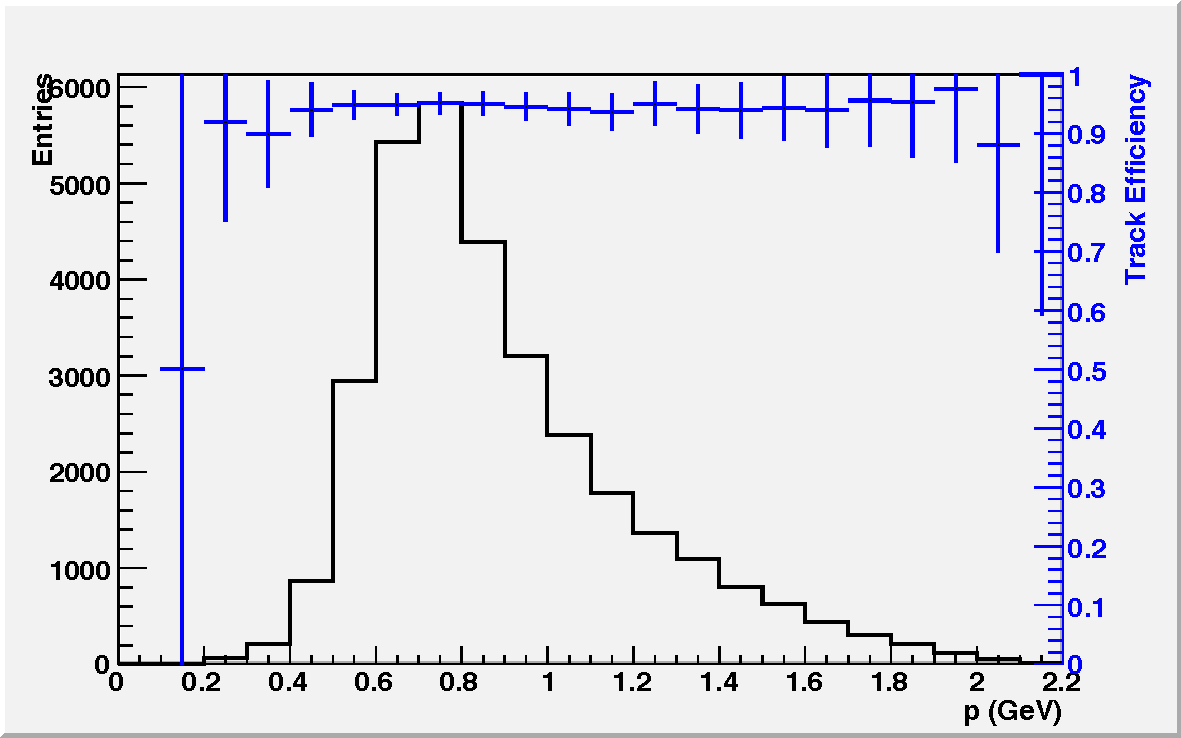
\includegraphics[scale=0.8]{performance/tracking_performance/pzE-Effic.pdf}
\caption{ Track reconstruction efficiency versus track momentum.  The blue histogram (right axis) show the track momentum distribution.  }
\label{fig:trkeffic}
\end{figure}

\begin{figure}
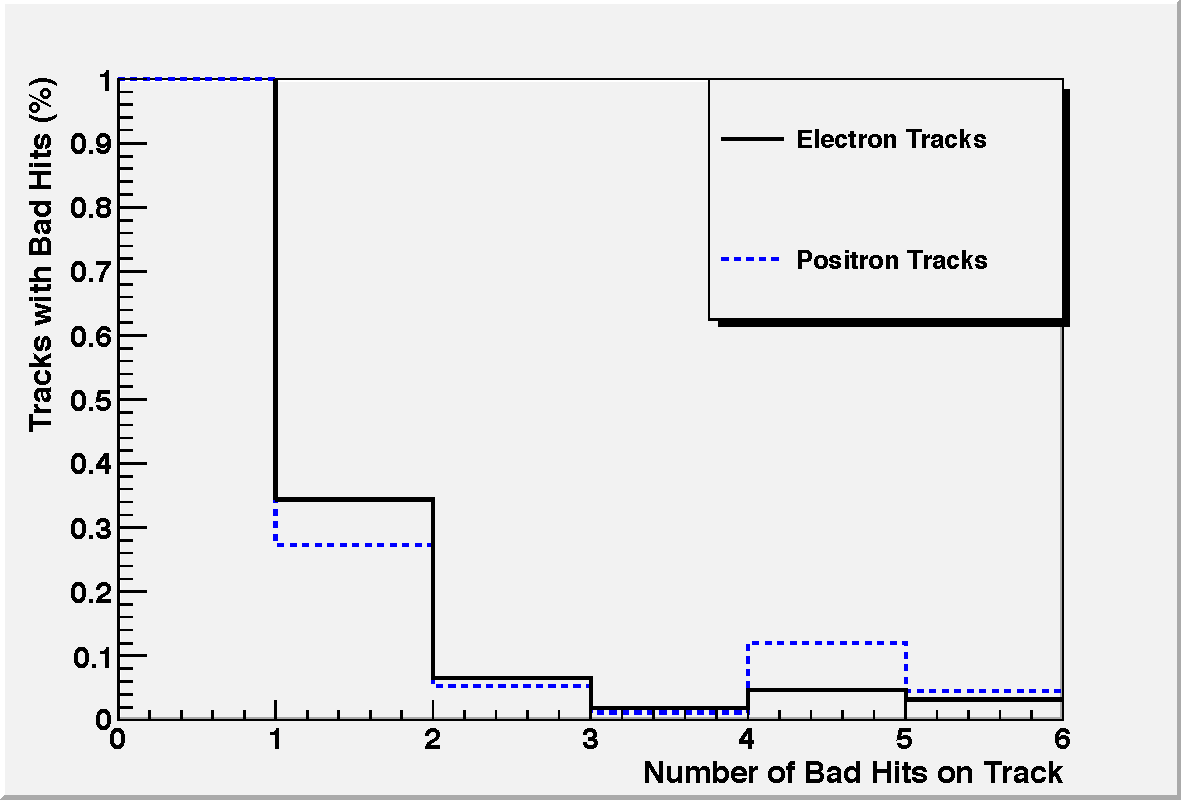
\includegraphics[scale=0.4]{performance/tracking_performance/nBadHits.pdf}
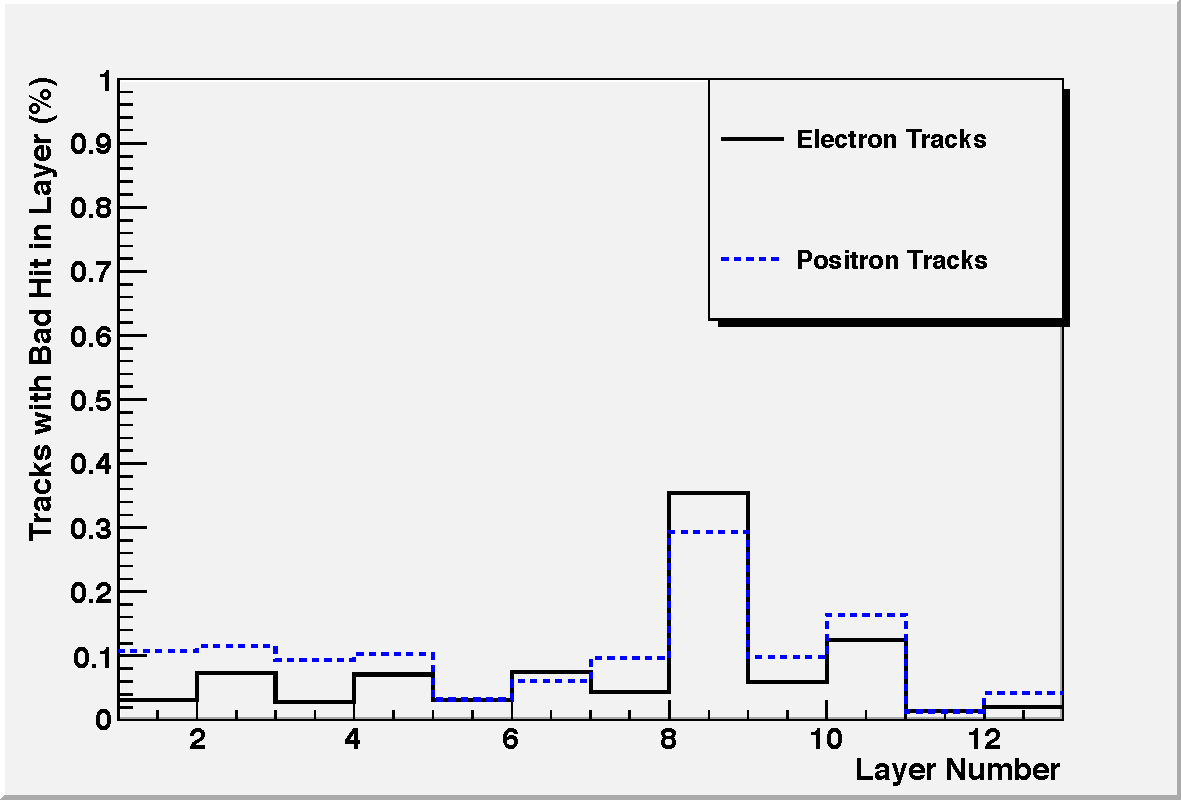
\includegraphics[scale=0.4]{performance/tracking_performance/BadLayer.pdf}
\caption{ The number of bad hits (left) and the layer number of the bad hit (right) 
for electron (black) and positron (blue) tracks.   }
\label{fig:badhits}
\end{figure}


\subsection{Track Momentum and Spatial Resolution}

The momentum resolution is shown in Figure \ref{fig:trkmom} as a function of momentum for tracks with 
0 bad hits and for tracks with one or more.  The momentum resolution for well-reconstructed 
tracks is $\delta p/p$ = 3.5\% (this is dependent on the beam energy and magnetic field) while for hits with bad hits it is slightly worse. 
%This momemtum 
%resolution is considerably worse than that in the full HPS proposal (~1.5\%) because small 
%angle stereo, which is used in the test run, provides much less precision in the bend plane 
%than the 90 degree stereo which is used in full HPS. The lower resolution still provides 
%adequate invariant mass resolution for this experiment.


\begin{figure}
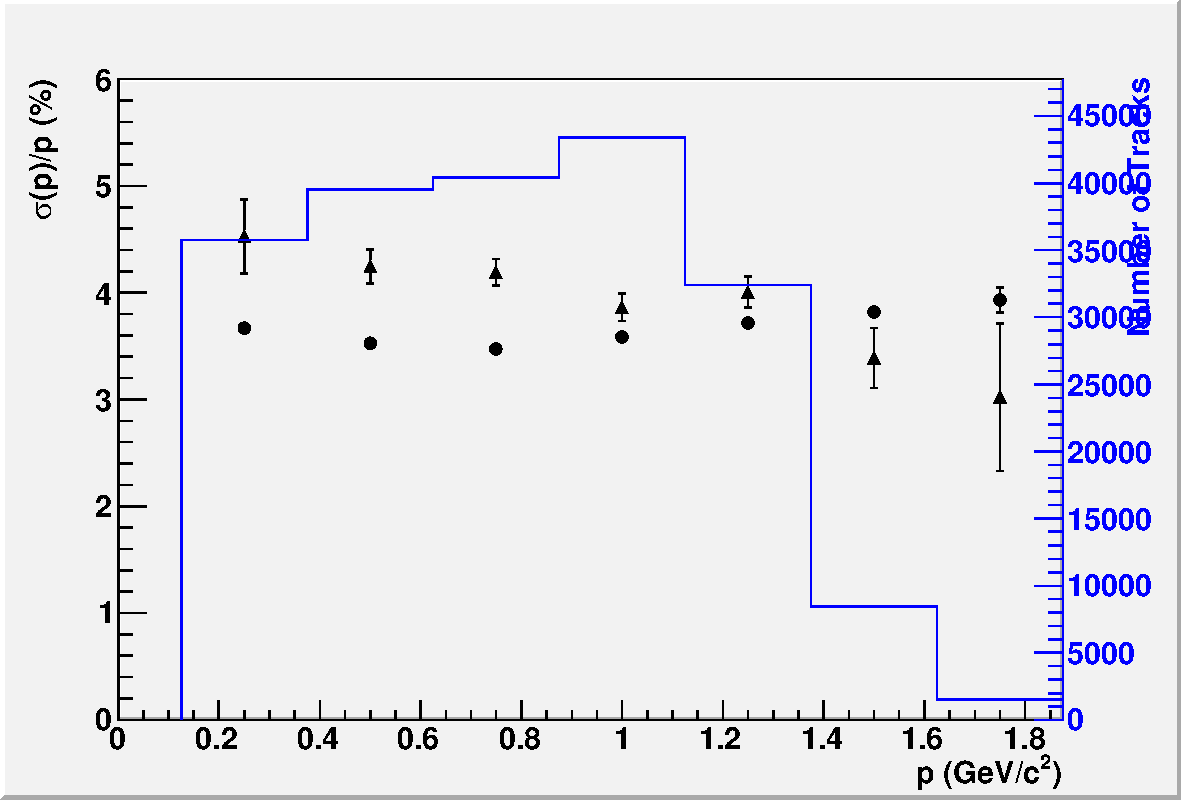
\includegraphics[scale=0.8]{performance/tracking_performance/momResvsMom.pdf}
\caption{  Fractional momentum resolution versus momentum. } 
\label{fig:trkmom}
\end{figure}


One quantity we use to determine track quality is the distance of closest approach (DOCA) 
to the beam axis.  We use this instead of the DOCA to the target beam spot since we are 
interested in long-lived decays and tracks from those will not point back to the target. 
We separate the distance into the bend plane (XOCA) and non-bend plane (YOCA) distances.  
Below, in Figure \ref{fig:doca}, is the resolution of these quantities as function of momentum.  
The resolution is, on average, about 100$\mu$m 300 $\mu$m) 
in the non-bend (bend) direction but increases significantly at low momentum.  The position 
resolution for tracks with one or more bad hits is somewhat worse, depending on which layer 
the bad hit is.  Tracks with bad hits in 
layers 1 or 2 are a major contribution to the tail of the vertex position distribution. 
    
For long lived A' decays, the position of the decay vertex is an important discriminating 
variable.  The dominant background to A' production is radiative events which originate 
in the target. Distinguishing A' decays from the background therefore depends on the vertex 
resolution and in particular on the tails of the vertex distribution. In order to study 
the tails, we use large samples of A' events decaying promptly overlaid on top of the 
simulated beam background events.
   
\begin{figure}
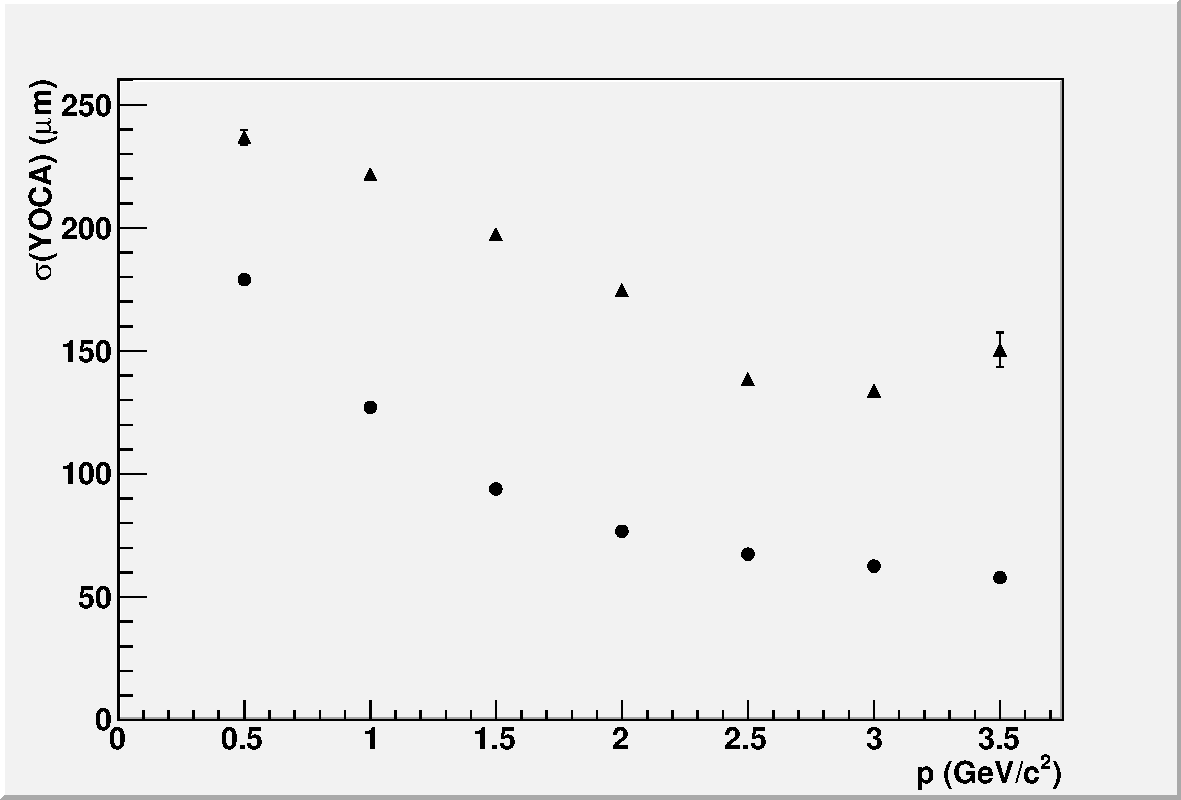
\includegraphics[scale=0.4]{performance/tracking_performance/yoca-MomResolution.pdf}
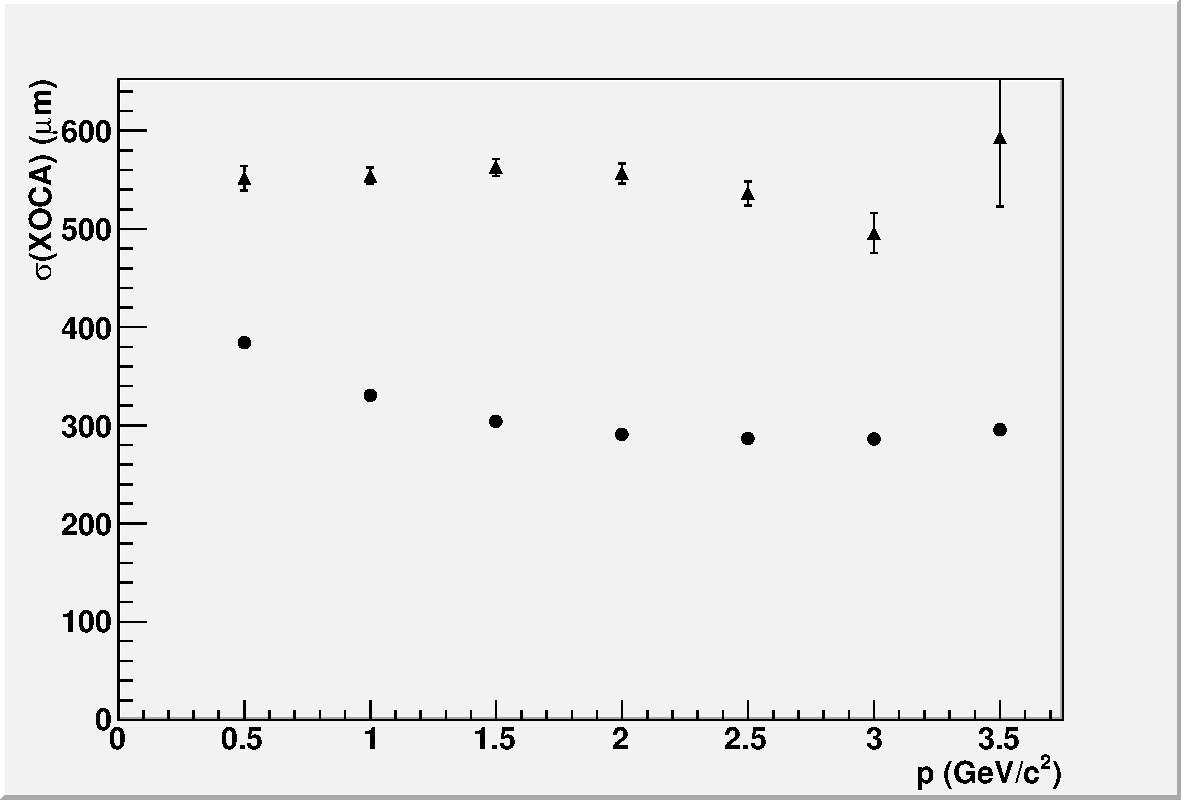
\includegraphics[scale=0.4]{performance/tracking_performance/xoca-MomResolution.pdf}
\caption{The resolution of the position of closest approach to the beam axis 
versus track momentum in the (left) non-bend direction and (right) bend direction.}
 \label{fig:doca}
\end{figure}

Each pair of oppositely charged tracks is fit to a common vertex using a Kalman filtering 
method first suggested by Billoir \cite{bf}, \cite{bq} and used in many experiments.  The method 
uses the measured helix parameters and their correlations to determine the most likely 
decay position of the A' and also returns fitted momenta for each particle.  We actually 
fit each pair twice with different hypotheses of their origin.  We constrain either 
the vertex to be consistent with an A':

\begin{itemize}
\item which originates in the 200$\mu$m $\times$ 40$\mu$m beamspot at the target, and moves off 
in the direction given by the measured A' momentum.  This fit will be used for the vertexing search.  
\item which originates and decays at the target within the 200$\mu$m $\times$ 40$\mu$m beamspot.  
This fit will be used for the bump-hunt only search.  
\end{itemize}

For each electron/positron pair reconstructed in the tracker, we compute the invariant mass based 
on the fitted momenta of the tracks.  The mass resolution depends on the invariant mass of the pair 
and is shown in Figure \ref{fig:massres}.  The closed circles  in Figure \ref{fig:massres} shows the improvement 
in the resolution for the second fit, where the decay is assumed to occur in the target.  

\begin{figure}
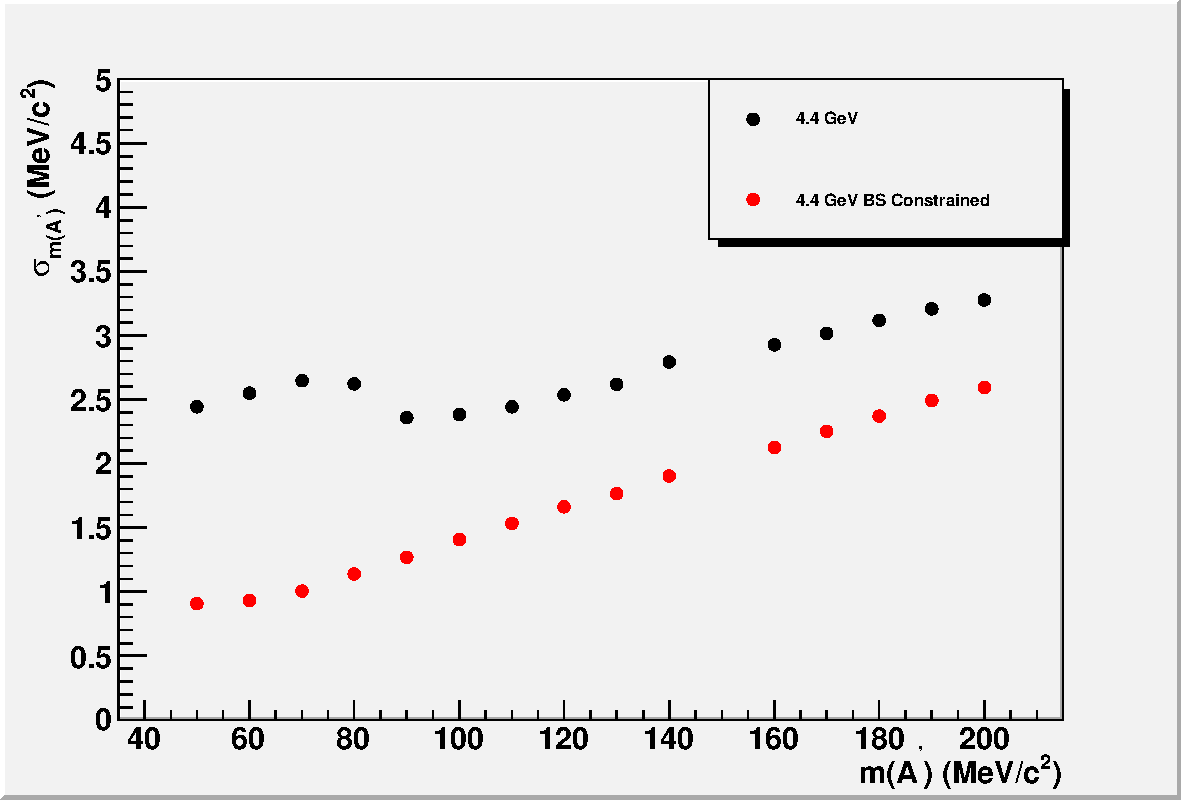
\includegraphics[scale=0.8]{performance/tracking_performance/massRes-4pt4.pdf}
\caption{The gaussian width of the mass distributions (MeV/c2) vs generated A' mass (MeV/c2). 
 The open circles are the resolutions when the decay is constrained to the target beamspot 
and the closed circles are without this constraint.    }
label{fig:massres}
\end{figure}



Even for prompt decays, the z vertex position (Vz) distribution of all reconstructed $e^+e^-$ pairs
  (solid black histogram, Figure \ref{fig:vtxResolutionRaw}) shows a long tail, still significant beyond 5cm.   
This tail is primarily comprised of events where one or both of the tracks use one or 
more bad hits.  Fortunately there are a number of quantities we can use to minimize the tails.  
Namely, for purposes of this proposal, we make the following cuts:

\begin{itemize}
\item The $\chi^2$  of each track is less than 20
\item The total momentum of the A' candidate is less than the beam energy
\item A very loose cut on the reconstructed vertex position $|V_x|<400\mu$m and $|V_y|<400\mu$m
\item The clusters in layer 1 of each track must be isolated from the next closest cluster by at least 500 $\mu$m 
\item A $\chi^2$ cut on the vertex fit of less than 5.
\end{itemize}

The vertex resolution depends on the invariant mass of the particles being vertexed. 
Lower masses have worse Gaussian resolutions as shown in Figure \ref{fig:vtxResolutionGauss}.  This is expected 
since the error on the opening angle ($\theta$), due to multiple scattering, scales like: 
 $\sigma (\theta )/\theta \sim (1/E)/(m/E) \sim 1/m$.
 
Figure \ref{fig:vtxResolutionRaw} shows the vertex resolution for samples of 80 MeV and 160 MeV A' events. 
The cuts above remove almost all of the tail past ~1.5cm (points with errors in Figure \ref{fig:vtxResolutionRaw}) 
while retaining ~50\% of the $e^+e^-$ pairs from the A' candidate. The events on the tail are 
enhanced with vertices where there are one or more bad hits on the track (represented by the 
blue histogram in Figure \ref{fig:vtxResolutionRaw}), although there is still a contribution from well-reconstructed 
tracks.  The rejection of tracks with bad hits depends strongly on the precision of the virtual A' 
trajectory, which in turn depends on the size of the beamspot. Having a beamspot significantly 
smaller than the intrinsic tracker resolution, 100$\mu$m in the non-bend and 300$\mu$m in 
the bend directions, is important.  

In practice, there is much more we can do to clean up the vertex and mass resolution both at 
the track level (e.g. remove hits that are clearly from scattered beam electrons) and at 
the vertex level.  These will be pursued in the near future.

\begin{figure}
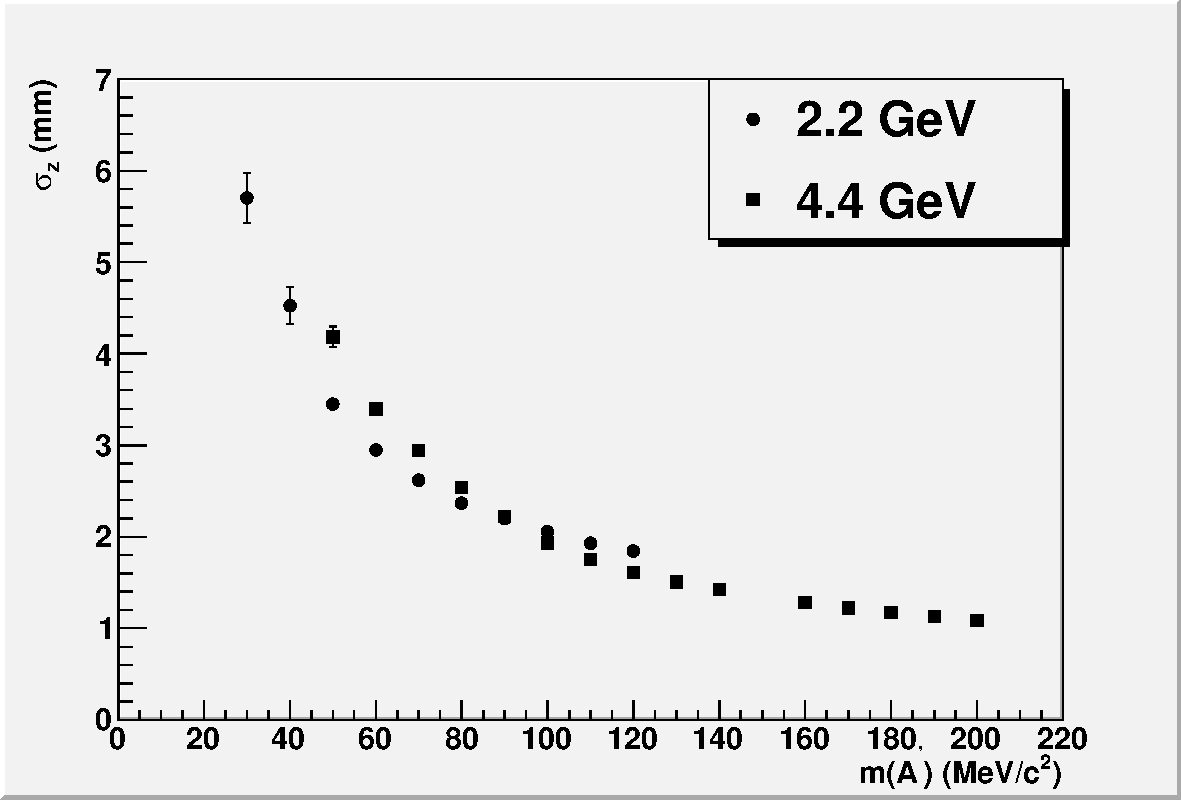
\includegraphics[scale=0.8]{performance/tracking_performance/vertexRes-4pt4-2pt2.pdf}
\caption{ The Gaussian resolution dependence versus $A^\prime$ mass for signal-only events.   }
\label{fig:vtxResolutionGauss}
\end{figure}
   

\begin{figure}
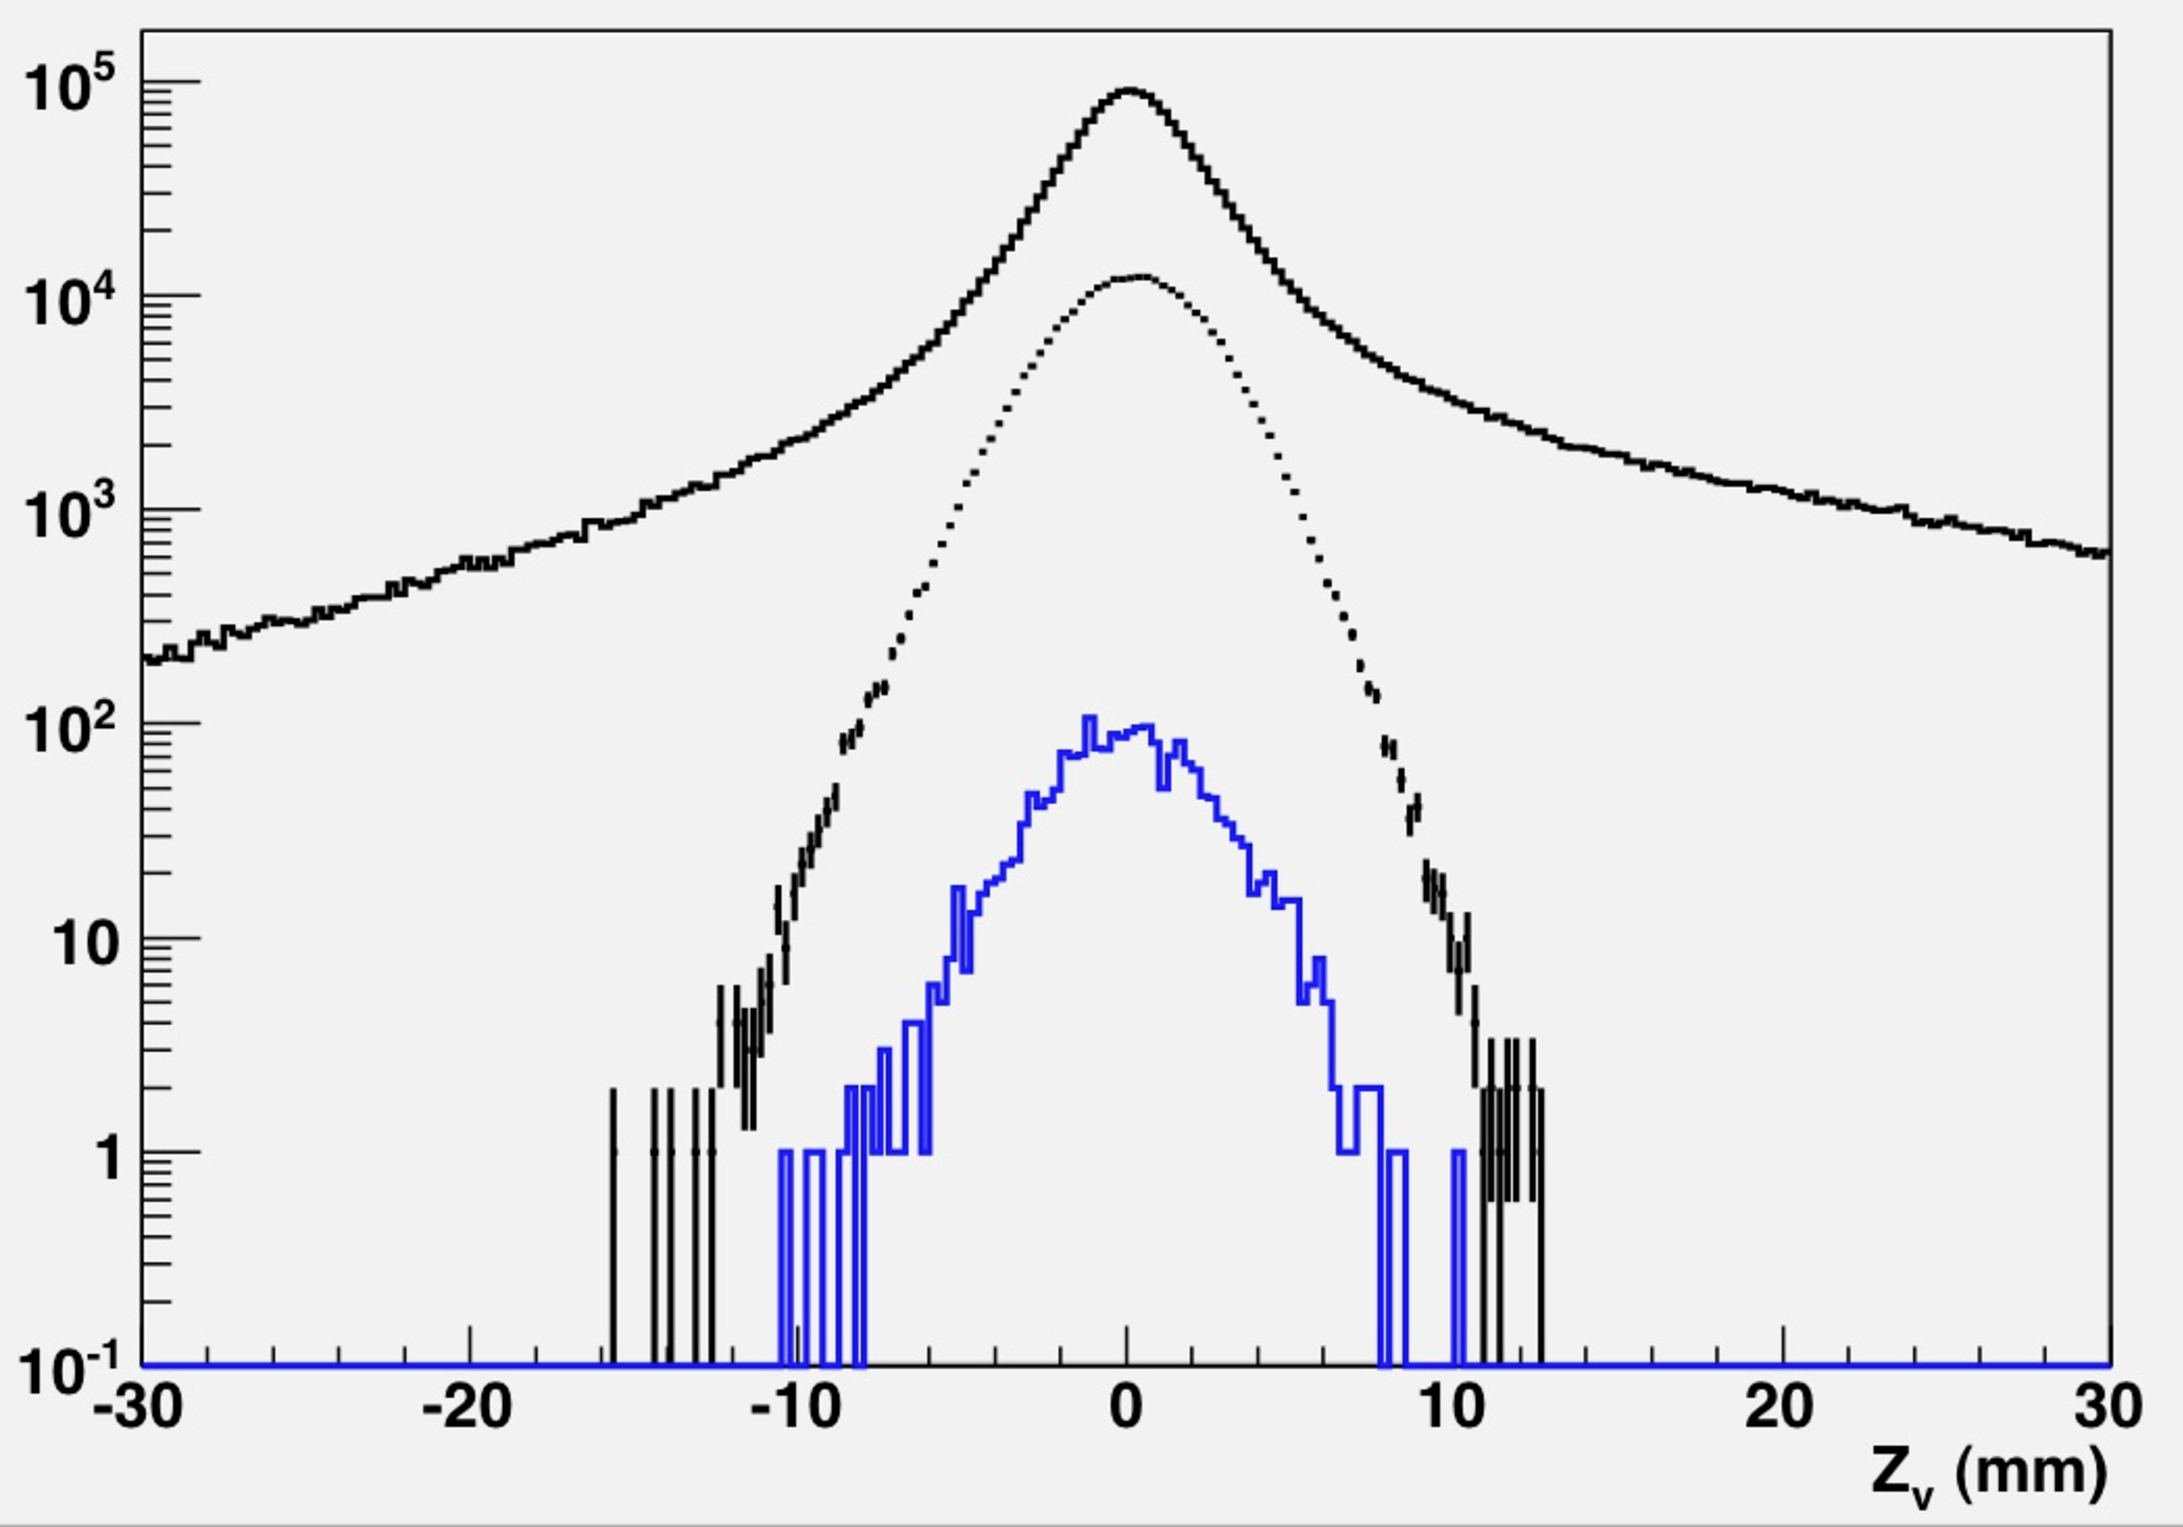
\includegraphics[width=0.8\textwidth]{performance/tracking_performance/v80.pdf}
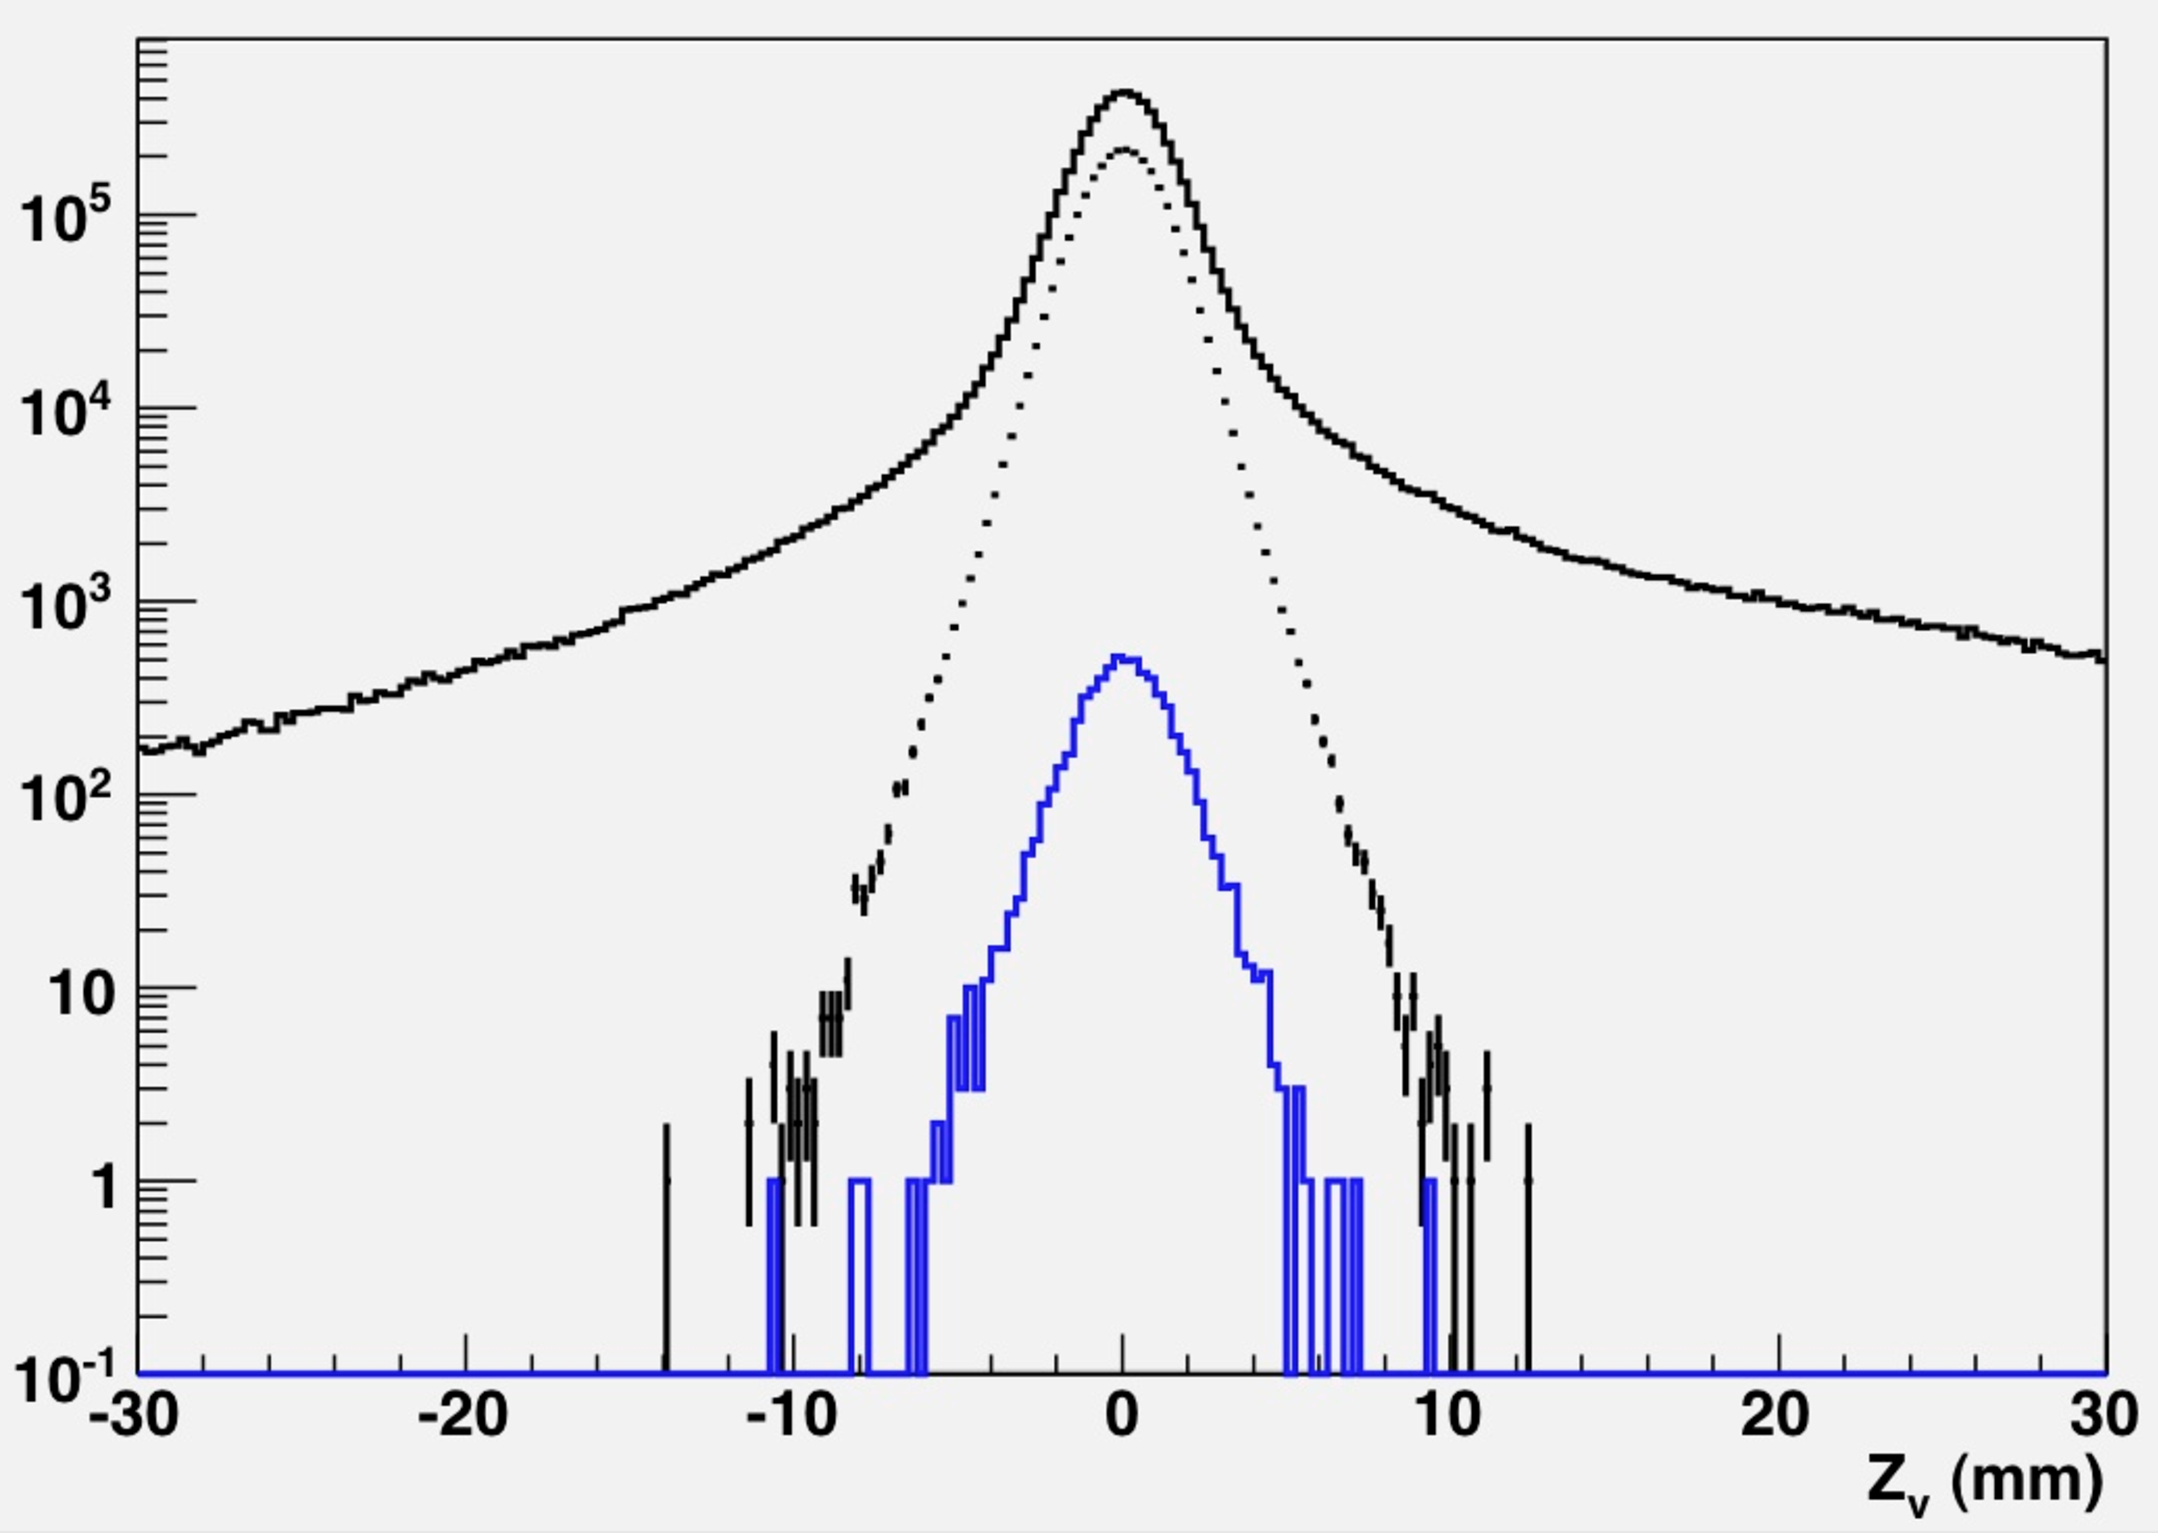
\includegraphics[width=0.8\textwidth]{performance/tracking_performance/v160.pdf}
\caption{Distribution of the reconstructed vertex position along the beam axis for 
4.4GeV 80MeV (top) and 160MeV (bottom) A' events before (solid black) and after (points 
with errors) selection.  The blue histogram shows the distribution for pairs that have 
at least one bad hit after selection.    }
\label{fig:vtxResolutionRaw}	
\end{figure}
  
